\subsection{Particelle doppie}

\begin{figure}
	\centering
	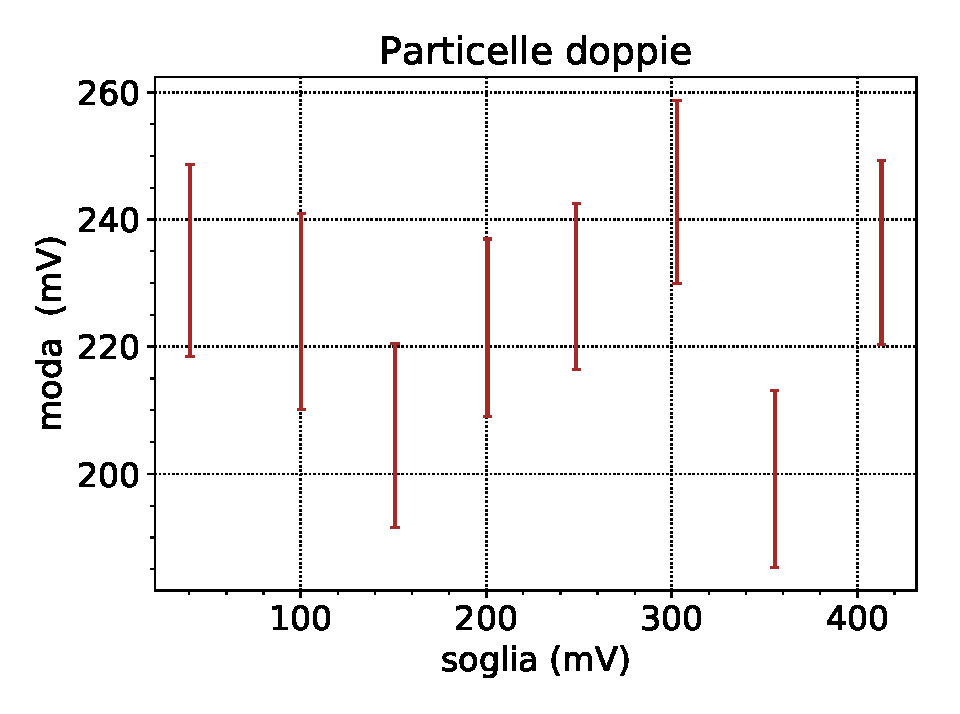
\includegraphics[width=23em]{doppie}
	\caption{Moda della distribuzione del rilascio di energia nel PM5
	negli eventi in coincidenza PM4 \& PM5
	in funzione della soglia del PM4.
	MODIFICA: \texttt{capsize=..., markersize=...}}
	\label{corre}
\end{figure}

Ci aspettiamo di osservare una distribuzione del rilascio di energia bimodale,
con una moda circa doppia dell'altra,
\marginpar{Mettere subito dopo angolo e collegare le cose.}
nel caso in cui ci sia un passaggio frequente di 2 particelle nello stesso momento.
Poiché non osserviamo questa caratteristica nella distribuzione del rilascio di energia,
\marginpar{Mettere questa misura cioè quella di 1\&6.}
proviamo con una strategia meno diretta.

Studiamo la distribuzione dell'energia rilasciata nel PM5,
per gli eventi in coincidenza 4\&5,
in funzione della soglia del PM4.
Un'eventuale presenza di eventi con particelle doppie,
quindi con distribuzione dell'energia rilasciata diversa,
provoca un cambiamento della distribuzione misurata in funzione della soglia.
Il PM5 ha la soglia più bassa possibile (\SI{30}{mV}) per mantenere minima la selezione.
La moda (calcolata con gli istogrammi) è riportata in \autoref{corre} in funzione della soglia.

Dalla \autoref{corre} non si nota un andamento.
Se avessimo avuto a disposizione due amplificatori
avremmo potuto analizzare le correlazioni temporali tra rilasci elevati di energia in due scintillatori diversi.
